\section{Macchina a stati finiti} \label{cap:FSM}
Il firmware implementato è stato formalizzato tramite una macchina a stati finiti (FSM). Un'automa a stati finiti è un modello matematico con cui è possibile descrivere, in modo preciso e sintetico, il comportamento di un sistema tramite un numero finito di stati, che rappresentano le condizioni operative nelle quali esso si può trovare. Il passaggio da uno stato all'altro avviene in seguito al verificarsi di particolari eventi e condizioni, che definiscono le \textit{funzioni di transizione}. Una caratteristica fondamentale delle FSM è la necessità di garantire l'unicità dello stato che, in un preciso istante di tempo, è attivo. Di conseguenza, è sempre possibile sapere con esattezza lo stato in cui si trova la macchina. Inoltre, è consentito effettuare solo una transizione alla volta. Per questo motivo, le transizioni da un particolare stato, che potrebbero potenzialmente attivarsi, devono essere mutuamente esclusive.
L'utilizzo di una macchina a numero finito di stati può essere adatto sia per la progettazione di un sistema sia per la descrizione di uno esistente. In particolare, è possibile modellare sistemi che sono:
\begin{itemize}
	\item dinamici, che evolvono cambiando stato nel tempo;
	\item discreti, cioè che le variabili in ingresso e gli stati del sistema si possono rappresentare con valori discreti;
	\item a simboli finiti, cioè che il numero di variabili in ingresso e gli stati può essere espresso con un numeri finito;
\end{itemize}
Una macchina a stati può essere rappresentata attraverso un grafo, in cui i nodi identificano gli stati e le transizioni sono rappresentate dagli archi.

Per entrambe le \textit{Adapter board} è stata progettata e implementata la medesima FSM. In particolare, sono stati identificati i seguenti stati:
\begin{enumerate}
	\setcounter{enumi}{-1}
	\item Start-up
	\item Idle
	\item Stream
	\item Error
\end{enumerate}
Nella figura \ref{fig:FSM} è stato riportato il grafo che descrive il comportamento della macchina a stati progettata e implementata.
\begin{figure}[b]
	\centering
	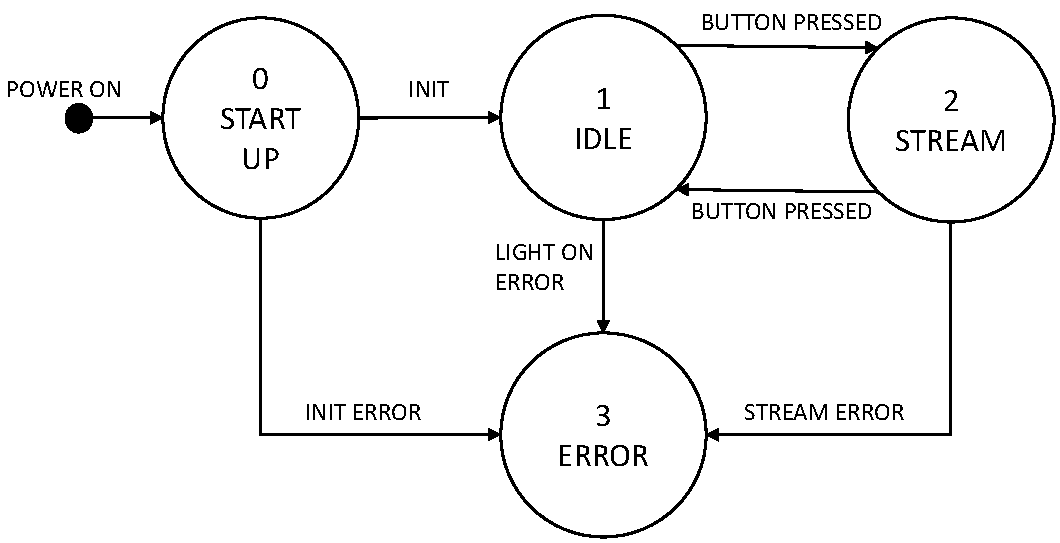
\includegraphics[width=0.6\linewidth]{ImageFiles/Macchina a stati finiti/FSM}
	\caption{Macchina a stati finiti del firmware delle due board progettate.}
	\label{fig:FSM}
\end{figure}

\paragraph{Start-up}
Lo stato di \textit{Start-up} rappresenta la fase di inizializzazione del sistema. Quando la board STM32F4DISCOVERY viene alimentata tramite una porta USB, il microcontrollore si avvia e entra nello stato di \textit{Start-up}. Si è scelto di associare ad ogni condizione del sistema un indicatore luminoso (uno dei quattro LED integrati sulla board) per segnalare all'utente lo stato attivo. Mentre il sistema si trova nello stato \textit{Start-up} il LED arancione rimane acceso. Vengono inizialmente configurate tutte le periferiche necessarie al funzionamento della comunicazione I\ap{2}C, della porta seriale USB e vengono inizializzati i pin GPIO. In particolare, sono inizializzate anche le strutture necessarie alle librerie HAL, presentate nella sezione~\ref{sec:Firmware}, fondamentali per la comunicazione I\ap{2}C e di tutte le librerie. Di seguito, viene effettuata la lettura del registro, appartenente al sensore PPG, che contiene il \textit{part-id} della scheda. Se non ci sono errori di lettura e l'identificativo acquisito rispetta le informazioni contenute nel datasheet del sensore, si può proseguire con l'inizializzazione della struttura dati nella quale saranno memorizzate tutte le informazioni per la configurazione del sensore. In caso di errore, il sistema andrà nello stato di \textit{Error}. A questo punto, vengono scritti i registri che determinano la configurazione del modulo PPG. Se l'operazione di scrittura avviene correttamente, il sistema può transitare nello stato di \textit{Idle}, altrimenti entra nello stato di \textit{Error}.
\paragraph{Idle}
Quando il sistema entra nello stato di \textit{Idle}, il LED arancio viene spento e si accende quello verde. Il sistema attende la pressione da parte dell'utente del pulsante, integrato sulla STM32F4DISCOVERY, che alla sua pressione il sensore PPG viene accesso (tramite la scrittura di un particolare registro) e il sistema transita nello stato di \textit{Stream}. Se la scrittura del registro non avviene con successo, il sistema viene portato nello stato di \textit{Error}.
\paragraph{Stream}
Nello stato di \textit{Stream}, il sistema continua ad eseguire due operazioni consecutive:
\begin{enumerate}
	\item lettura dei dati acquisiti dalla FIFO interna al sensore;
	\item invio tramite interfaccia USB dei dati letti.
\end{enumerate}
I campioni acquisiti dal sensore PPG vengono recuperati tramite la lettura del registro \textit{FIFO\_DATA} che permette di accedere alla FIFO dove vengono memorizzati temporaneamente le misurazioni effettuate dal sensore. Tuttavia, la dimensione del registro è di 1 byte mentre quella delle acquisizioni sono di \SI{19}{\bit} ciascuna, pari alla risoluzione dell'ADC. Per questo motivo, per ottenere il valore acquisito di un campione è necessario effettuare tre letture consecutive del registro, per un totale di 24 byte letti. \`E necessario quindi applicare la maschera \textbf{0x07} sul primo byte letto cosicché il valore dei primi \SI{5}{\bit}, che non contengono informazioni rilevanti, vengano ignorati. Più precisamente, solamente il sensore MAXM86161 valorizza i primi \SI{5}{\bit} con un'informazione rilevante. Infatti, essi rappresentano un \textit{tag} che identifica il contenuto dei byte successivi. Confrontando il valore del tag letto e i valori riportati nel datasheet, si è in grado di capirne il significato. Per cui, durante la lettura dei campioni dal sensore MAXM86161 si è introdotto un controllo sul tag per assicurasi che il valore letto corrisponda alla misurazione dell'intensità luminosa del LED corretto. Il sensore MAXM86161 presenta tre LED (rosso, infrarosso e verde). Per questo motivo, è necessario effettuare tre letture consecutive del registro \textit{FIFO\_DATA} per ottenere il valore di un campione acquisito per ogni LED, per un totale di 9 byte per ogni ciclo di lettura. Il sensore MAX86916 presenta invece quattro LED (rosso, infrarosso, verde e blu) e necessita quindi di effettuare quattro letture, per un totale di 12 byte.

I dati letti vengono temporaneamente memorizzati in un buffer, in attesa dell'invio al computer collegato. Affinché sia possibile inviare tramite USB i campioni letti, è necessario stabilire il formato dei messaggi che il microcontrollore invia al computer collegato, definendo così un semplice protocollo di comunicazione. Nelle tabelle \ref{tab:USBByteMAX86916} e \ref{tab:USBByteMAXM86161} sono mostrati i formati dei messaggi rispettivamente per la board con il sensore MAX86916 e MAXM86161. 
\begin{table}[t]
	\newcolumntype{C}{>{\centering\arraybackslash}p{2em}}
	\centering
	\begin{tabular}[c]{|l|C|C|C|C|C|C|C|C|C|}
		\hline
		BIT   & 0 & 1 & 2 & 3         & 4         & 5         & 6 & 7        & 8 
		\\ \hline
		VALORE & ? & ! & 0 & IR{[}0{]} & IR{[}1{]} & IR{[}2{]} & 0 & R{[}0{]} & R{[}1{]} \\ 
		\hline
	\end{tabular}

	\vspace{0.5cm}
		
	\begin{tabular}[c]{|l|C|C|C|C|C|C|C|C|C|}
		\hline
		BIT & 9        & 10 & 11       & 12       & 13       & 14 & 15       & 16       & 17       \\ \hline
		VALORE & R{[}2{]} & 0  & G{[}0{]} & G{[}1{]} & G{[}2{]} & 0  & B{[}0{]} & B{[}1{]} & B{[}2{]} \\ \hline
	\end{tabular}
	\caption{Struttura del messaggio inviato tramite USB della board con il sensore MAX86916.}
	\label{tab:USBByteMAX86916}
\end{table}

\begin{table}[t]
	\newcolumntype{C}{>{\centering\arraybackslash}p{2em}}
	\centering
	\begin{tabular}[c]{|l|C|C|C|C|C|C|C|}
		\hline
		BIT   & 0 & 1 & 2 & 3         & 4         & 5         & 6 
		\\ \hline
		VALORE & ? & ! & 0 & G{[}0{]} & G{[}1{]} & G{[}2{]} & 0 \\ \hline
	\end{tabular}
	
	\vspace{0.5cm}
	
	\begin{tabular}[c]{|l|C|C|C|C|C|C|C|}
		\hline
		BIT & 7        & 8 & 9       & 10       & 11       & 12 & 13  \\ \hline
		VALORE & IR{[}0{]} & IR{[}1{]}  & IR{[}2{]} & 0 & R{[}0{]} & R{[}1{]}  & R{[}2{]} \\ \hline
	\end{tabular}
	\caption{Struttura del messaggio inviato tramite USB della board con il sensore MAXM86161.}
	\label{tab:USBByteMAXM86161}
\end{table}
\noindent Come indicato nelle tabelle, i primi due byte contengono i caratteri ("!?") che identificano l'inizio del messaggio. Successivamente, vengono inseriti i valori acquisiti dalla FIFO (tre byte per ogni LED). Si utilizza la convezione \textit{Big Endian} per la trasmissione dei byte.

Come mostrato in \Fig\ref{fig:FSM}, il sistema permane nello stato \textit{Stream} fino a quando l'utente non preme nuovamente il pulsante oppure si verifica un errore durante la lettura dei dati dal sensore o l'invio dei messaggi tramite USB. Se si verifica un errore, il sistema transita nello stato di \textit{Error}. Se invece viene premuto il pulsante, il sistema torna nello stato di \textit{Idle}. Mentre il sistema si trova in questo stato, solamente il LED blu rimane acceso.

\paragraph{Error} Il sistema si trova nello stato di \textit{Error} a seguito del verificarsi di un errore durante il funzionamento. Per questo motivo, tutte le operazioni di lettura e scrittura, sia con il sensore PPG sia tramite USB, vengono inibite e per utilizzare nuovamente il sistema è necessario spegnere e riaccendere la board. Lo stato viene indicato all'utente tramite l'accensione del LED rosso presente sulla STM32F4DISCOVERY. 

\clearpage